\section{Auswertung}
\label{sec:Auswertung}

\subsection{Statische Methode}

In \autoref{fig:45grad1} ist zu erkennen, dass beide Temperaturen ähnlich verlaufen, doch ist die Temperatur am Abtastpunkt T4 durchschnittlich 11.908\% kleiner.

\begin{figure}
    \centering
    \includegraphics[scale=0.7]{build/plot1.pdf}
    \caption{Die Temperaturverläufe von Messing  weisen eine ähnliche logarithmische Steigung auf. Dabei steigt T4 langsamer an als T1.}
    \label{fig:45grad1}
\end{figure}

%\newpage
Sehr ähnlich verlaufen auch die Temperaturen in \autoref{fig:45grad2}, wobei hier T5 deutlich stärker ansteigt als T8.
Die Temperaturkurven haben einen durchschnittlichen Unterschied von 27.499\% voneinander.

\begin{figure}
    \centering
    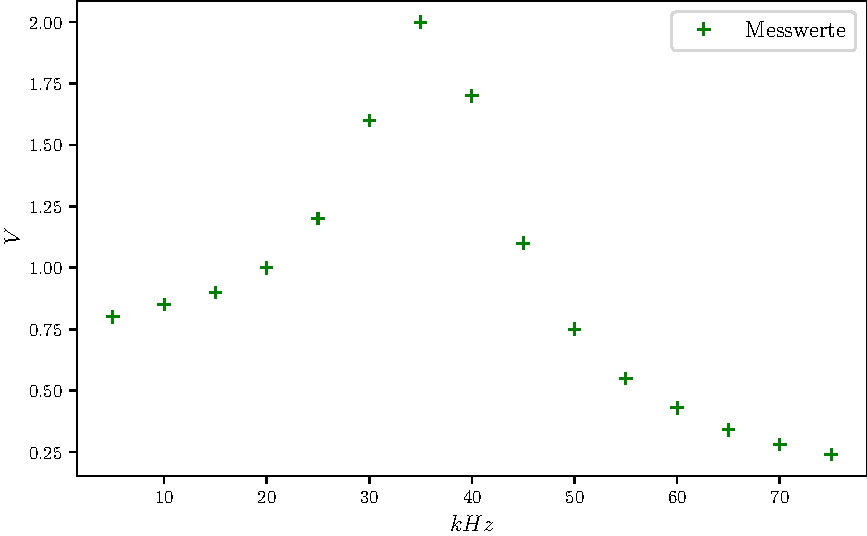
\includegraphics[scale=0.7]{build/plot2.pdf}
    \caption{Die Temperaturverläufe von Aluminium und Edelstahl steigen ebenfalls logarithmisch an, wobei Edelstahl deutlich langsamer an Hitze gewinnt.}
    \label{fig:45grad2}
\end{figure}
%\newpage
Die Temperatur der Thermoelemente am Ende der Messung bei $425\ s$ betragen:

\begin{itemize}
    \centering
    \item[] $T1 = 48.74\ °C$ 
    \item[] $T4 = 50.14\ °C$
    \item[] $T5 = 50.37\ °C$
    \item[] $T8 = 35.64\ °C$
\end{itemize}

Die beste Wärmeleitung hat demnach Aluminium am Abgriff T5.\\
Um den Wärmestrom $\Delta Q/\Delta t$ zu berechnen, braucht es die Werte der Wärmeleitfähigkeit für die verschiedenen Materialien \cite{web}, sowie den Querschnitt der Metalle und den Abstand der Abgriffstellen.
\begin{itemize}
    \centering
    \item[] $\kappa_{Messing} = 111\ \frac{W}{m\cdot K}$
    \item[] $A_{Messing(breit)} = 48\cdot 10^{-6}\ m^2$
    \item[] $\Delta x_{Messing(breit)} = 0.03\ m$ 
    \item[] 
    \item[] $\kappa_{Edelstahl} = 14.4\ \frac{W}{m\cdot K}$
    \item[] $A_{Edelstahl} = 48\cdot 10^{-6}\ m^2$
    \item[] $\Delta x_{Edelstahl} = 0.03\ m$ 
\end{itemize}

Daraus ergeben sich für 5 zufällige Messzeiten mithilfe der \autoref{eq:warmcurrent} folgende Wärmeströme in \autoref{tab:warmcurrent}.

\begin{table}
    \centering
    \caption{Tabelle des Wärmestroms für 5 versch. Messzeiten.}
    \begin{tabular}{c|c|c|c|c}
        \toprule
        Messzeit [s] & $\Delta T = T2\ -\ T1$ [K] & $\frac{\Delta Q}{\Delta t}_{12}\ [W]$ & $\Delta T = T7\ -\ T8$ [K] & $\frac{\Delta Q}{\Delta t}_{78}\ [W]$\\
        \midrule
        50 & 5.73 & -1.02 & 5.17 & -0.119\\
        100 & 5.32 & -0.94 & 9.19 & -0.212\\
        150 & 4.48 & -0.796 & 10.51 & -0.242\\
        200 & 3.87 & -0.687 & 10.69 & -0.246\\
        250 & 3.42 & -0.607 & 10.48 & -0.241\\
    \end{tabular}
    \label{tab:warmcurrent}
\end{table}

\begin{figure}
    \centering
    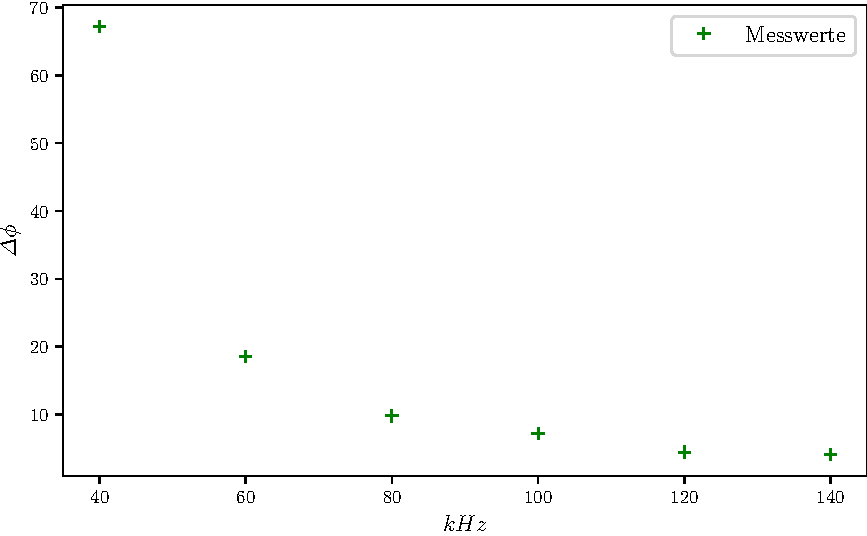
\includegraphics[scale=0.7]{build/plot3.pdf}
    \caption{Plot der Differenzen der Temperatur von Messing und Edelstahl.}
    \label{fig:deltaT}
\end{figure}

\newpage
